% =====================================================================
%  Internship Report — Farah AYARI
%  A Governed Intelligence for Islamic Banking
%  The Integrated RAGLab & Bank Assistant Platform
%
%  Engineering Report — 15-20 pages
%  Compilation: pdflatex (2 passes) + compile on Overleaf
%  Assets in ./assets/ — no exotic dependencies
%  Arabic terms are transliterated so it compiles with pdflatex without Arabic fonts
% =====================================================================
\documentclass[a4paper,12pt]{report}
\usepackage[utf8]{inputenc}
\usepackage[T1]{fontenc}
\usepackage[english]{babel}
\usepackage{graphicx}
\usepackage{geometry}
\usepackage{setspace}
\usepackage{hyperref}
\usepackage{float}
\usepackage{array}
\usepackage{booktabs}
\usepackage{xcolor}
\usepackage{titlesec}
\usepackage{fancyhdr}
\usepackage{tikz}
\usepackage{tcolorbox}
\usepackage{enumitem}
\usepackage{amsmath}
\usepackage{caption}
\usepackage{wrapfig}
\usepackage{eso-pic}
\usetikzlibrary{calc, shadows, fadings, positioning, decorations.pathreplacing}

\geometry{margin=2.3cm, top=2.6cm, bottom=2.2cm}
\setstretch{1.30}
\graphicspath{{./assets/}{./}}

% ── Custom colors — Al Baraka + ESPRIT universe ───────────────────────
\definecolor{abarakaRed}{HTML}{E0122F}
\definecolor{abarakaOrange}{HTML}{F5881C}
\definecolor{abarakaDark}{HTML}{0A1931}
\definecolor{espritNavy}{HTML}{1B2A4E}
\definecolor{espritRed}{HTML}{C1272D}
\definecolor{softGray}{HTML}{F5F7FB}
\definecolor{midGray}{HTML}{E8ECF3}
\definecolor{accentGold}{HTML}{B57A14}
\definecolor{accentTeal}{HTML}{1F7A5C}
\definecolor{textDark}{HTML}{1A1F2E}

\definecolor{chapterBlue}{HTML}{1B2A4E}
\definecolor{chapterRed}{HTML}{E0122F}

% ── Personal info ─────────────────────────────────────────────────────
\newcommand{\StudentName}{Farah AYARI}
\newcommand{\SchoolName}{Private Higher School of Engineering and Technology --- ESPRIT}
\newcommand{\CompanyName}{Al Baraka Bank Tunisia}
\newcommand{\CompanySite}{Centre Urbain Nord, Tunis}
\newcommand{\SupervisorName}{Mrs.\ Ahlem Ben Haddoud}
\newcommand{\AcademicYear}{2025 -- 2026}
\newcommand{\ReportTitleA}{A Governed Intelligence}
\newcommand{\ReportTitleB}{for Islamic Banking}
\newcommand{\ReportSubtitle}{The Integrated RAGLab \& Bank Assistant Platform}
\newcommand{\ReportTagline}{A retrieval-augmented system where every answer is traceable, every \\ refusal is honest, and every decision is auditable}
\newcommand{\DegreeName}{Engineering Degree --- Software Engineering}

% ── Hyperref ───────────────────────────────────────────────────────────
\hypersetup{
  colorlinks=true,
  linkcolor=chapterBlue,
  urlcolor=abarakaRed,
  citecolor=chapterBlue,
  pdfauthor={Farah AYARI},
  pdftitle={Internship Report — A Governed Intelligence for Islamic Banking},
  pdfsubject={ESPRIT — Al Baraka Bank Tunisia}
}

% ── Title formatting ──────────────────────────────────────────────────
\titleformat{\chapter}[display]{\bfseries\color{chapterBlue}\Huge}{}{0pt}{\Huge\vspace{-0.3cm}}[\vspace{0.15cm}\hrule height 1.2pt\vspace{0.2cm}]
\titlespacing{\chapter}{0pt}{-6pt}{14pt}
\titleformat{\section}{\bfseries\color{chapterBlue}\Large}{\thesection}{0.6em}{}
\titleformat{\subsection}{\bfseries\color{textDark}\large}{\thesubsection}{0.6em}{}
\titleformat{\subsubsection}{\bfseries\color{textDark}\normalsize}{\thesubsubsection}{0.6em}{}

% ── Fancy header/footer ───────────────────────────────────────────────
\pagestyle{fancy}
\fancyhf{}
\fancyhead[L]{\small \color{midGray!60!black} \textit{Farah AYARI --- ESPRIT $\cdot$ Al Baraka Bank}}
\fancyhead[R]{\small \thepage}
\fancyfoot[C]{\tiny \color{midGray!60!black} Internship Report --- Centre Urbain Nord --- \SupervisorName}
\renewcommand{\headrulewidth}{0.25pt}
\renewcommand{\footrulewidth}{0pt}

% ── Helper: colored box ───────────────────────────────────────────────
\newtcolorbox{highlightbox}[1]{
  colback=softGray, colframe=chapterBlue!25, boxrule=0.6pt, arc=3pt,
  left=6pt, right=6pt, top=5pt, bottom=5pt, title=#1,
  fonttitle=\bfseries\small\color{chapterBlue}, coltitle=chapterBlue,
  colbacktitle=softGray
}
\newtcolorbox{problembox}[1]{
  colback=white, colframe=abarakaRed!35, boxrule=0.7pt, arc=3pt,
  left=7pt, right=7pt, top=6pt, bottom=6pt, title=#1,
  fonttitle=\bfseries\small\color{abarakaRed}, coltitle=abarakaRed,
  colbacktitle=white
}
\newcommand{\inlineTag}[1]{\colorbox{abarakaRed!10}{\small\bfseries\color{abarakaRed}#1}}

% ── Document start ────────────────────────────────────────────────────
\begin{document}

% ══════════════════════════════ COVER PAGE ═════════════════════════════
\begin{titlepage}
% --- Background layers ---
\begin{tikzpicture}[remember picture, overlay]
  % Full page white base
  \fill[white] (current page.south west) rectangle (current page.north east);
  % Top decorative band (red → orange gradient simulated with multiple rects)
  \fill[abarakaRed] ($(current page.north west)+(0,0)$) rectangle ($(current page.north east)+(0,-3.8cm)$);
  \fill[abarakaRed!85!abarakaOrange] ($(current page.north west)+(0,-3.8cm)$) rectangle ($(current page.north east)+(0,-4.05cm)$);
  \fill[abarakaOrange] ($(current page.north west)+(0,-4.05cm)$) rectangle ($(current page.north east)+(0,-4.85cm)$);
  % Bottom thin bands
  \fill[espritNavy] ($(current page.south west)+(0,0)$) rectangle ($(current page.south east)+(0,1.45cm)$);
  \fill[abarakaRed] ($(current page.south west)+(0,1.45cm)$) rectangle ($(current page.south east)+(0,1.65cm)$);
  % Subtle diagonal accent (opacity simulated)
  \fill[white, opacity=0.09] ($(current page.north east)+(0,-4.85cm)$) -- ++(-13cm,-8cm) -- ++(0,8cm) -- cycle;
  % Decorative dots
  \foreach \x in {1,2,...,6}{
    \fill[white, opacity=0.18] ($(current page.north east)+(-1.2cm - \x*0.7cm, -1.15cm)$) circle (1.1pt);
  }
\end{tikzpicture}

% --- Top white text on red band ---
\vspace*{-0.9cm}
\begin{center}
{\small\color{white}\bfseries\scshape Republic of Tunisia}\\[1pt]
{\footnotesize\color{white!92} Ministry of Higher Education and Scientific Research}\\[0.15cm]
{\tiny\color{white!88} \SchoolName\ \ {\color{white}$\bullet$} \ CompanyName\ ---\ \CompanySite}
\end{center}

\vspace{0.35cm}

% --- Logos row (placeholder frames with text, replaced by images if available) ---
\begin{center}

\begin{tikzpicture}
  % ESPRIT logo placeholder — left
  \node[draw=white!40, fill=white, rounded corners=3pt, minimum width=5.2cm, minimum height=2.1cm, inner sep=4pt] (esprit) at (-4.5,0) {
    \begin{minipage}{4.6cm}\centering
      \IfFileExists{assets/esprit-tunisia-logo-private-engineering--1.png}{
        \includegraphics[width=3.6cm,height=1.45cm,keepaspectratio]{assets/esprit-tunisia-logo-private-engineering--1.png}
      }{
        \IfFileExists{assets/esprit-ariana.jpg}{
          \includegraphics[width=3.6cm,height=1.45cm,keepaspectratio]{assets/esprit-ariana.jpg}
        }{
          {\small\bfseries\color{espritNavy} ESPRIT}\\{\tiny\color{espritNavy} Private Higher School of\\ Engineering \& Technology}
        }
      }\\
      {\tiny\color{espritNavy!70} \textit{Ariana --- est. 2003}}
    \end{minipage}
  };
  % Separator
  \draw[white!35, line width=0.4pt] (-1.4,-1.05) -- (-1.4,1.05);
  % Al Baraka logo placeholder — right
  \node[draw=white!40, fill=white, rounded corners=3pt, minimum width=5.2cm, minimum height=2.1cm, inner sep=4pt] (baraka) at (4.5,0) {
    \begin{minipage}{4.6cm}\centering
      \IfFileExists{assets/al-baraka-bank-tunisia-logo-red-orange-1.png}{
        \includegraphics[width=3.6cm,height=1.45cm,keepaspectratio]{assets/al-baraka-bank-tunisia-logo-red-orange-1.png}
      }{
        \IfFileExists{assets/albaraka-front.png}{
          \includegraphics[width=3.6cm,height=1.45cm,keepaspectratio]{assets/albaraka-front.png}
        }{
          {\small\bfseries\color{abarakaRed} Al Baraka Bank}\\{\tiny\color{abarakaRed!80} Your Partner Bank}
        }
      }\\
      {\tiny\color{abarakaRed!70} \textit{Islamic Banking since 1983}}
    \end{minipage}
  };
\end{tikzpicture}
\end{center}

\vspace{0.55cm}

% --- Main title block ---
\begin{center}
{\footnotesize\color{espritNavy!75}\scshape\bfseries Internship Report \quad$\vert$\quad End-of-Studies Project}\\[0.38cm]
{\Huge\bfseries\color{chapterBlue} \ReportTitleA}\\[0.12cm]
{\Huge\bfseries\color{abarakaRed} \ReportTitleB}\\[0.35cm]
{\large\color{textDark!85}\textit{\ReportSubtitle}}\\[0.35cm]
% tagline in box

\begin{tikzpicture}
  \node[fill=softGray, rounded corners=4pt, inner sep=8pt, draw=midGray, line width=0.4pt] {
    \begin{minipage}{13.5cm}\centering
      \footnotesize\color{textDark!78}\textit{\ReportTagline}
    \end{minipage}
  };
\end{tikzpicture}\\[0.45cm]
% Subject tag
{\small\color{white}\colorbox{chapterBlue}{\ \ Final-Year Engineering Internship \quad$\vert$\quad \DegreeName\ \ }}\\[0.25cm]
{\small\color{espritNavy!72}\textit{Architecture, integration and governance of a banking RAG platform}}
\end{center}

\vspace{0.45cm}

% --- Student / Supervisor info in elegant card ---
\begin{center}

\begin{tikzpicture}
\node[fill=white, draw=midGray, rounded corners=5pt, inner sep=0, drop shadow={shadow xshift=1.5pt, shadow yshift=-1.5pt, opacity=0.10}] (card) {
\begin{minipage}{14.2cm}
\vspace{6pt}
\begin{tabular}{p{4.0cm} p{9.6cm}}
\small\bfseries\color{espritNavy} Student &
  \small\color{textDark} \StudentName\ --- \SchoolName \\[3pt]
\small\bfseries\color{espritNavy} Host Organization &
  \small\color{textDark} \CompanyName\ --- \CompanySite \\[3pt]
\small\bfseries\color{abarakaRed} Supervisor &
  \small\color{textDark} \SupervisorName\ --- Advisor, Al Baraka Bank (Centre Urbain Nord) \\[3pt]
\small\bfseries\color{espritNavy} Academic Year &
  \small\color{textDark} \AcademicYear\qquad{\color{midGray}$\vert$}\qquad \small\color{espritNavy!75} \textit{ESPRIT --- Software Engineering} \\
\end{tabular}
\vspace{6pt}
\end{minipage}
};
% small red accent line on left of card
\fill[abarakaRed] ($(card.north west)+(0,-0.22cm)$) rectangle ($(card.south west)+(0.12cm,0.22cm)$);
\end{tikzpicture}
\end{center}

\vfill

% --- Bottom bar text (on navy background) ---
\begin{center}
{\footnotesize\color{white!90} \textbf{Trust through traceability} \quad$\cdot$\quad Every answer cites its source \quad$\cdot$\quad Every refusal explains why}\\[0.12cm]
{\tiny\color{white!72} No account identifiers, repository URLs, or credentials appear in this report by design. All figures are traceable to frozen benchmark artifacts.}
\end{center}
\vspace{0.15cm}

\end{titlepage}
% ════════════════════════════ END COVER ════════════════════════════════

% ── Dedication ─────────────────────────────────────────────────────────
\clearpage
\thispagestyle{empty}
\vspace*{2.2cm}
\begin{center}
{\Large\bfseries\color{chapterBlue} Dedication}\\[0.25cm]
{\color{abarakaRed}\rule{3.2cm}{1.1pt}}\\[0.6cm]
\end{center}
\begin{quote}
\centering
\large\itshape\color{textDark!88}
``To my family, whose unwavering support made this journey possible,\\[3pt]
to \textbf{\color{chapterBlue}Mrs.\ Ahlem Ben Haddoud}, whose guidance, rigor and trust shaped every decision in this work,\\[3pt]
and to everyone who believes that technology, when governed,\\[3pt]
can serve trust.''\\[0.7cm]
\normalsize\upshape\normalfont\color{textDark!75}
\StudentName\ --- \SchoolName
\end{quote}

\vspace{1.2cm}
\begin{center}
{\Large\bfseries\color{chapterBlue} Acknowledgments}\\[0.25cm]
{\color{abarakaRed}\rule{3.2cm}{1.1pt}}\\[0.6cm]
\end{center}
\begin{quote}
\small\color{textDark!85}
I express my deepest gratitude to \textbf{\color{chapterBlue}\SupervisorName}, my internship supervisor at \textbf{\CompanyName{} --- \CompanySite}, for her availability, her precise feedback, and the clarity of her decisions. At every critical junction --- from the choice of the corpus to the final engine switch --- her judgment turned a technical possibility into a responsible banking feature.

I thank the teams of Al Baraka Bank for their welcome, the documents they entrusted to this project, and the operational feedback that revealed defects invisible in tests.

I thank the faculty of \textbf{ESPRIT} for the training that made this project possible, and in particular for the emphasis on measurable engineering over mere demonstration.

\vspace{0.35cm}
\begin{center}
{\footnotesize\color{espritNavy!70}\textit{The Centre Urbain Nord headquarters in Tunis --- where product, compliance and IT decisions converge --- provided the ideal ground for building a system where correctness matters more than fluency.}}
\end{center}
\end{quote}

% ── Abstract ───────────────────────────────────────────────────────────
\clearpage
\chapter*{Abstract}
\addcontentsline{toc}{chapter}{Abstract}
\markboth{Abstract}{Abstract}

\begin{highlightbox}{In one paragraph}
In regulated banking, a wrong answer about a rate, a fee or a deadline is not a minor inaccuracy --- it is a legal risk. This internship delivered a complete, governed and measurable answer: an integrated platform where a bank-operated web application consumes a dedicated RAG (Retrieval-Augmented Generation) intelligence engine, both designed to \textbf{never invent figures or rules}. The report focuses only on what was built, why it was built this way, and what was learned when reality tested it.
\end{highlightbox}

The platform comprises two cooperating systems. \textbf{RAGLab} is a document-grounded question-answering engine over four real Arabic banking documents (Law 2016-48, BCT Circular 2019-08, an internal Islamic-operations guide, and a training primer on Islamic finance). Every claim it produces is backed by a \textbf{verbatim quote} whose numbers must literally appear in the source; when evidence is insufficient, it refuses honestly and explains what is missing. \textbf{Bank Assistant} is a trilingual (French / Arabic / English) customer and staff web application (Angular 21 + Spring Boot 4 + PostgreSQL) that owns the relational schema, authentication, quotas, persistence and audit, and calls RAGLab over an authenticated, streaming-aware internal contract.

Together they form a clean separation: the edge handles identity, governance and regulation; the intelligence engine handles retrieval, grounding and generation --- stateless, auditable and versioned. This report tells that story through architecture, measured results and the problems that were solved along the way. No dates are needed to understand it; ideas are.

\vspace{0.4cm}
\noindent\textbf{Keywords:} {\small Retrieval-Augmented Generation $\cdot$ Islamic Banking $\cdot$ Grounded Answers $\cdot$ Citation Verification $\cdot$ Arabic NLP $\cdot$ Spring Boot $\cdot$ Angular $\cdot$ System Architecture $\cdot$ AI Governance}

\vspace{0.35cm}
\noindent\textbf{Résumé (Français):} {\small Ce rapport présente une plateforme bancaire intégrée où une application web opérée par la banque consomme un moteur d'intelligence RAG gouverné. Chaque réponse est traçable jusqu'à sa source, chaque refus est motivé, et chaque décision est auditable --- parce qu'en banque, une réponse fausse sur un taux n'est pas une imprécision, c'est un risque juridique.}

\vspace{0.35cm}
\noindent\textbf{Note on content:} {\footnotesize\color{textDark!75} This report contains no account identifiers, repository URLs or credentials. All figures cited are traceable to frozen benchmark artifacts in the two repositories. The document is written around ideas and architecture, not a chronology.}

% ── Table of Contents ──────────────────────────────────────────────────
\clearpage
\tableofcontents
\clearpage

% ══════════════════════════ CHAPTER 1 ══════════════════════════════════
\chapter{Host Organization: Al Baraka Bank Tunisia}

\section{Identity and History}

\textbf{Al Baraka Bank Tunisia} is the first Islamic bank in Tunisia and the Maghreb. Created on \textbf{15 June 1983} as \textit{Beit Ettamouil Tounsi Saoudi --- BEST Bank} by the Tunisian State and Sheikh Saleh Abdallah Kamel (founder of the Dallah Al Baraka Group), it changed its name to \textbf{Al Baraka Bank Tunisia} in 2009 as part of the unification of the Al Baraka Group identity. In 2013, it obtained approval to transform from a non-resident bank into a \textbf{universal resident bank}, allowing it to serve individuals, professionals and enterprises with Sharia-compliant products.

The Group itself, \textbf{Al Baraka Group B.S.C.}, headquartered in Bahrain Bay, operates over 600 branches in 12 countries (Jordan, Egypt, Tunisia, Sudan, Bahrain, Turkey, South Africa, Algeria, Lebanon, among others) and is one of the pioneers of participative finance worldwide.

Today the bank operates \textbf{44 branches} across Tunisia, with its modern headquarters at the \textbf{Centre Urbain Nord} in Tunis --- one of the capital's largest economic hubs. It has been elected \textbf{Best Islamic Bank in Tunisia (2018, 2019, 2021)} and honored with \textbf{five awards at the IFN Awards 2024}.

\section{A Sharia-Compliant Product Universe}

The bank's offerings operate within \textbf{Tunisian Law No.\ 2016-48 of 11 July 2016} on banks and financial institutions, which explicitly defines Islamic banking operations (Articles 12--16) and entrusts the \textbf{Central Bank of Tunisia (BCT)} with regulating their compliance via circulars such as \textbf{Circular BCT No.\ 2019-08} --- two documents that form the very corpus this project is built upon.

\begin{table}[H]
\centering\small
\begin{tabular}{p{4.2cm}p{10.0cm}}
\toprule
\textbf{Family} & \textbf{Products} \\
\midrule
Trading \& Investment & \textit{Murabaha} (cost-plus sale), \textit{Salam} (deferred delivery), \textit{Istisna'a} (manufacturing), \textit{Mudaraba} / \textit{Musharaka} (partnership), \textit{Sukuk}, participative investment deposits \\
Leasing \& Financing & \textit{Ijara} with acquisition option, \textit{Beit Al Baraka} (home ownership), \textit{Tas'heelat} (personal finance), equipment \& working-capital financing \\
International \& Daily & Documentary credits, remittances, leasing, day-to-day banking \\
\bottomrule
\end{tabular}
\caption{Product families at Al Baraka Bank Tunisia (Centre Urbain Nord catalog).}
\end{table}

\section{The Internship Site}

\begin{tcolorbox}[colback=softGray, colframe=abarakaRed!28, boxrule=0.5pt, arc=3pt, left=6pt, right=6pt, top=5pt, bottom=5pt]
\small
\textbf{\color{abarakaRed}Al Baraka Bank --- Centre Urbain Nord Branch}\\
\small Avenue Cheikh Mohamed Fadhel Ben Achour, Centre Urbain Nord, 1082 Tunis\\
Tel: (+216) 71 183 203 \quad$\vert$\quad Head office: +216 71 18 65 00 \quad$\vert$\quad SWIFT: BEITTNTT\\[2pt]
\normalsize\small
\textit{The Centre Urbain Nord is not merely an address; it is the bank's operational heart, where product, compliance and IT decisions converge --- and where this project was supervised by Mrs.\ Ahlem Ben Haddoud.}
\end{tcolorbox}

% ══════════════════════════ CHAPTER 2 ══════════════════════════════════
\chapter{Project Vision: A Governed Banking Intelligence}

\section{The Business Problem}

Banks produce and consume vast amounts of regulatory and procedural text: laws, central-bank circulars, internal guides, training materials. Finding a reliable answer in these documents is expensive, and entrusting it to a raw language model is dangerous: a generative model always answers, even when it does not know, and nothing distinguishes a copied sentence from an invented one.

Three concrete tensions motivated the project:

\begin{enumerate}[leftmargin=1.2cm, itemsep=3pt]
\item \textbf{The user's question is rarely the document's question.} A customer asks in everyday language (\textit{``can I open a shop?''}) where the corpus uses technical terms (\textit{sigha, mahal al-aqd, tamwil}). The answer must be found despite this lexical gap.
\item \textbf{Multilingual asymmetry.} The corpus is in Arabic, but questions arrive in French and English. A French question must be answerable from an Arabic passage without ever translating the user or the document.
\item \textbf{Errors are costly.} In banking, a false rate, deadline or sanction is a legal exposure --- not a minor imprecision.
\end{enumerate}

\section{The North Star: Five Properties}

The product was defined with five properties, in strict priority order:

\begin{table}[H]
\centering\small
\begin{tabular}{clp{9.5cm}}
\toprule
\textbf{\#} & \textbf{Property} & \textbf{What it means in practice} \\
\midrule
1 & \textbf{Grounded \& Auditable} & Every answer traceable to a source; nothing fabricated about rates or terms \\
2 & \textbf{Compliant} & PII scrubbed on the way out; no learning from customer chats \\
3 & \textbf{Quota-Controlled \& Secure} & Public channel metered; intelligence engine unreachable from Internet \\
4 & \textbf{Regulable by Staff} & Admins edit taxonomy, governed facts and documents \\
5 & \textbf{Multilingual} (Arabic RTL first-class) & French/Arabic/English questions, Arabic RTL layout \\
\bottomrule
\end{tabular}
\caption{North-star properties that governed every technical choice.}
\end{table}

\section{What Was Delivered: Two Systems, One Product}

\begin{center}
\begin{tcolorbox}[colback=white, colframe=chapterBlue!30, boxrule=0.6pt, arc=4pt, width=14.5cm, left=8pt, right=8pt, top=8pt, bottom=8pt]
\small
\textbf{\color{chapterBlue}RAGLab} \textit{answers}; \textbf{\color{abarakaRed}Bank Assistant} \textit{serves customers and governs what RAGLab knows.} Neither writes into the other's store. The bank's staff sees every conversation from its first message (Java persists before calling the engine), and a customer never sees which document an answer came from. That boundary is what makes the answer path auditable.
\end{tcolorbox}
\end{center}

\noindent The web app exposes a public landing page, a floating assistant widget, an authenticated client portal (accounts, cards, transactions, simulations), and an eleven-screen admin back-office including a five-tab RAGLab Console. The intelligence engine is a versioned, stateless HTTP microservice with 25+ routes, a frozen contract, and a full audit trail.

% ══════════════════════════ CHAPTER 3 ══════════════════════════════════
\chapter{System Architecture: The Full Picture}

\section{End-to-End Flow}

\begin{figure}[H]
\centering
\IfFileExists{assets/architecture_schema.png}{
  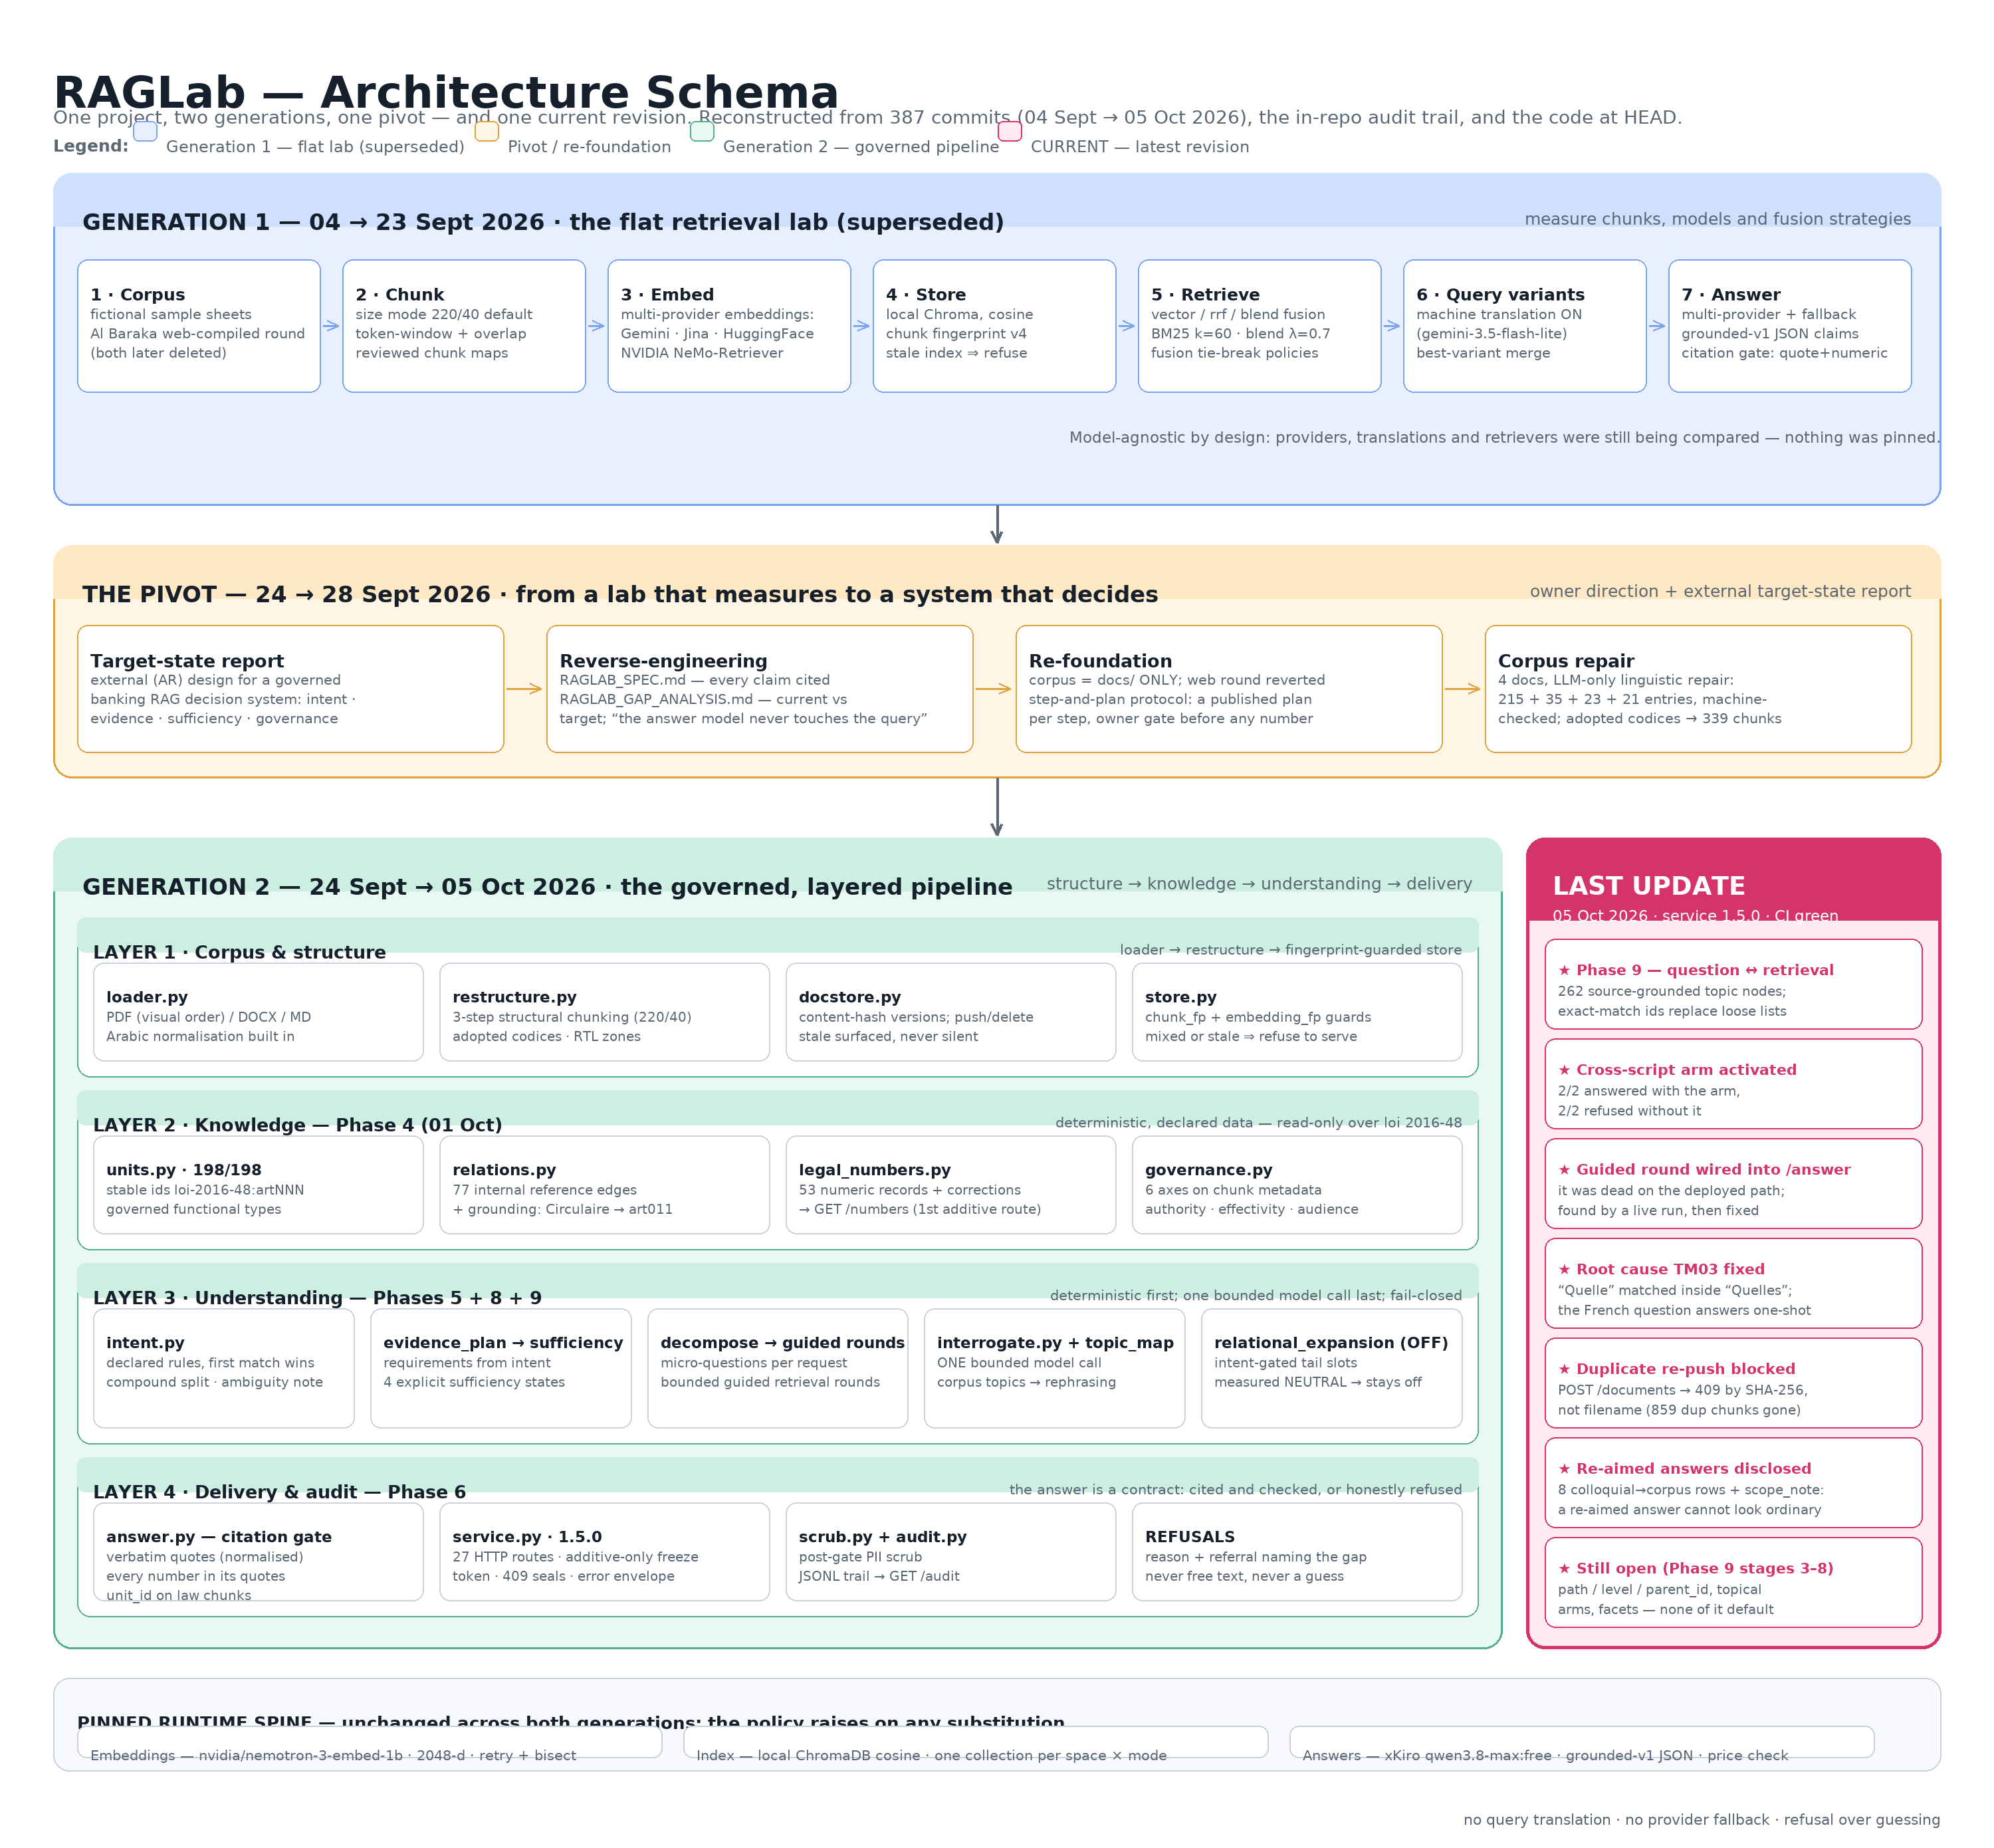
\includegraphics[width=0.97\textwidth]{assets/architecture_schema.png}
  \caption{Full architecture: from browser to intelligence. Generation 1 (flat lab), the pivot, Generation 2 (four governed layers), and the current update. The engine is external and addressed by \texttt{ip:port}.}
  \label{fig:arch}
}{
  \fbox{\parbox{0.9\textwidth}{\centering\textit{Architecture diagram: browser $\rightarrow$ nginx $\rightarrow$ Spring Boot edge $\rightarrow$ RAGLab $\rightarrow$ Postgres \\ (see assets/architecture\_schema.png)}}}
\end{figure}

\noindent In words:

\begin{center}
\small
\begin{tabular}{p{2.8cm}l}
\toprule
\textbf{Layer} & \textbf{Responsibility} \\
\midrule
Browser $\rightarrow$ nginx & Angular SPA; security headers; \texttt{/api} proxy; Server-Sent Events \\
nginx $\rightarrow$ Spring Boot & JWT auth, role checks, quotas, persistence, admin; owns the relational schema (Flyway) \\
Spring Boot $\rightarrow$ RAGLab & \texttt{POST \{RAGLAB\_URL\}/answer} with shared \texttt{X-Service-Token}; masked context; streaming relay \\
RAGLab & Retrieval $\rightarrow$ grounded answer $\rightarrow$ citation + numeric gates; returns text + claims + sources \\
Database & PostgreSQL (Flyway, \texttt{ddl-auto=validate}); 15 migrations; single writer \\
\bottomrule
\end{tabular}
\end{center}

\noindent\textbf{Key separation:} the \textit{business schema} (users, sessions, messages, documents, quotas) belongs to \textbf{Java + Flyway}. The \textit{vector index} belongs to the \textbf{Python agent}. No shared-DB write coupling. This is not a convenience --- it is the design that makes audit possible.

\section{Technology Stack at a Glance}

\begin{table}[H]
\centering\footnotesize
\begin{tabular}{p{3.0cm}p{5.2cm}p{5.8cm}}
\toprule
\textbf{Layer} & \textbf{Choice} & \textbf{Why this, not that} \\
\midrule
Frontend & Angular 21 (standalone), Vitest, self-hosted Inter & SPA with lazy modules; no Google-fonts build dependency \\
Backend Edge & Java 21, Spring Boot 4, Flyway, JWT, virtual threads & Edge must own schema with \texttt{validate}; virtual threads prevent carrier pinning \\
Intelligence & Python 3.11, FastAPI + uvicorn, explicit code & No LangChain/LlamaIndex --- every behavior readable \\
Vector Store & ChromaDB local + BM25 (k1=1.5, b=0.75) & Local avoids cloud cost \& banking-data egress; fingerprint guards against stale serving \\
Embeddings / LLM & NVIDIA \texttt{nemotron-3-embed-1b} (2048-d) + xKiro \texttt{qwen/qwen3.8-max:free} & Measured best on Arabic corpus; two pinned models, zero fallback \\
Tokenization & \texttt{tiktoken} \texttt{cl100k\_base} + fallback & Exact budget; fingerprint encodes tokenizer \\
Persistence & PostgreSQL, Redis queue, Flyway & Single schema owner; Redis BRPOP durable queue \\
Deployment & Docker Compose, \texttt{Dockerfile.prod}, offline tarball & Same images dev $\rightarrow$ prod; Windows-native path \\
\bottomrule
\end{tabular}
\caption{Stack choices: sobriety as a governance decision.}
\end{table}

This sobriety is intentional: \textbf{no orchestration framework, no external vector DB, no vendor SDK in the repository} --- the entire behavior is legible for audit.

\section{The Two Lifecycles}

\begin{itemize}[leftmargin=1.2cm, itemsep=2pt]
\item \textbf{Document lifecycle:} pushed to RAGLab via \texttt{POST /documents} (content-hash versioned; identical bytes = no-op; SHA-256 dedup), then batch-indexed with \texttt{POST /ingest} (one job at a time; \texttt{409} is a state, not an error). The edge's \texttt{documents} table holds a parallel record but no longer drives indexing --- RAGLab owns its index and reports it honestly (\texttt{pending / indexed / stale}).
\item \textbf{Conversation lifecycle:} browser $\rightarrow$ edge (quota gate) $\rightarrow$ RAGLab (retrieval $\rightarrow$ generation $\rightarrow$ gate) $\rightarrow$ edge (scrub $\rightarrow$ persist $\rightarrow$ settle quota $\rightarrow$ stream). The edge opens the exchange row \textbf{before} calling the engine so even a failure is visible to staff.
\end{itemize}

Figure~\ref{fig:workflow} shows the chat path as the customer experiences it.

\begin{figure}[H]
\centering
\IfFileExists{assets/workflow.png}{
  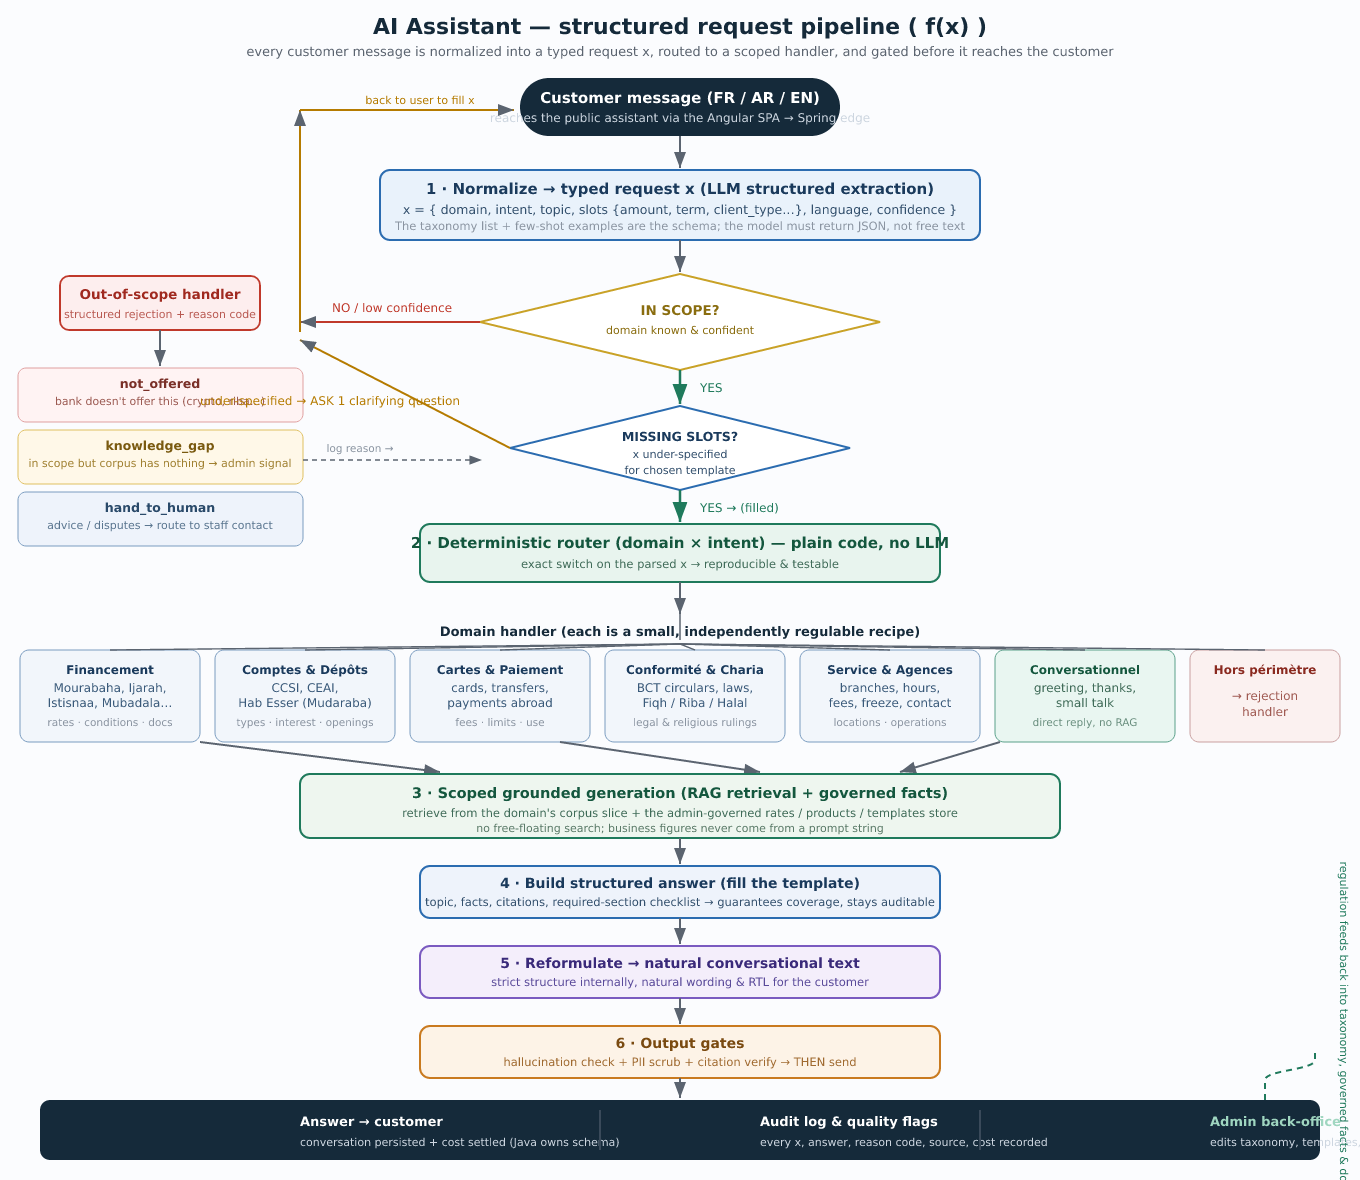
\includegraphics[width=0.92\textwidth]{assets/workflow.png}
  \caption{Customer chat path: two-phase metering, streaming, and persistence. The edge is the single writer.}
  \label{fig:workflow}
}{
  \fbox{\parbox{0.85\textwidth}{\centering\textit{Workflow diagram (assets/workflow.png)}}}
}
\end{figure}

% ══════════════════════════ CHAPTER 4 ══════════════════════════════════
\chapter{The Intelligence Engine --- RAGLab}

\section{Corpus and the Arabic Challenge}

The evaluation corpus is \textbf{four real, unabridged Arabic documents}:

\begin{table}[H]
\centering\small
\begin{tabular}{p{6.2cm}p{3.2cm}c}
\toprule
\textbf{Document} & \textbf{Role} & \textbf{Fragments} \\
\midrule
Law 2016-48 (198 articles, 11 titles) & Superior legal reference & 233 \\
BCT Circular 2019-08 (20 chapters) & Operational framing & 13 \\
Internal Islamic Operations Guide & Internal policy \& compliance & 54 \\
Introduction to Islamic Finance (\textit{Madkhal}) & Training, definitions & 39 \\
\midrule
\textbf{Total} & & \textbf{339} \\
\bottomrule
\end{tabular}
\caption{The governed corpus: four real documents, 339 structure-aware fragments.}
\end{table}

\noindent The PDFs are scanned legal Arabic: visual-order lines, reversed word order, corrupted digits, broken headings --- unusable without repair. See \S\ref{sec:problems} for how this was solved.

\section{Structure-Aware Chunking}

Two chunkers are implemented and measured. The legacy \texttt{size} mode (220 tokens + 40 overlap) remains; the adopted \texttt{restructure} mode dominates:

\begin{enumerate}[leftmargin=1.2cm, itemsep=2pt]
\item \textbf{Semantic normalization} --- gazette header cleanup, repeated-header dropping ($\geq$3 occurrences), section-marker extraction (\textit{al-fasl / al-bab / al-qism}), visual-order Arabic repair by zone, hierarchy into Markdown (\texttt{\#}, \texttt{\#\#}, \texttt{\#\#\#}).
\item \textbf{Breadcrumb enrichment} --- injecting \texttt{h1 > h2 > h3} context above every heading and table, so a chunk carries its ancestry.
\item \textbf{Recursive structural splitting} over \texttt{["\textbackslash n\# ", "\textbackslash n\#\# ", "\textbackslash n\#\#\# ", "\textbackslash n\textbackslash n", "\textbackslash n", " "]} at the same 220/40 budget.
\end{enumerate}

Each chunk carries an \textbf{identity card}: \texttt{document}, \texttt{chunk\_index}, \texttt{heading}, \texttt{language}, \texttt{section\_type}, \texttt{chunk\_fp} (fingerprint v4), \texttt{embedding\_fp}, \texttt{embedding\_model}.

\begin{tcolorbox}[colback=accentTeal!08, colframe=accentTeal!35, boxrule=0.5pt, arc=3pt]
\small \textbf{Measured impact:} Structural chunking gains \textbf{+20 points of hit@1} over window splitting (live: 51 $\rightarrow$ 71; offline BM25: 42 $\rightarrow$ 62) --- the single largest architectural win.
\end{tcolorbox}

\section{Embeddings and Storage}

\begin{itemize}[leftmargin=1.2cm, itemsep=2pt]
\item \textbf{Model:} \texttt{nvidia/nemotron-3-embed-1b}, native \textbf{2048 dimensions}, via NVIDIA Build endpoint (batch 32, exponential backoff + \texttt{Retry-After}, bisect on degenerate vectors, resumable cache).
\item \textbf{Store:} one \textbf{ChromaDB persistent collection per (embedding-space $\times$ chunking mode)}, \texttt{hnsw:space=cosine}. BM25 lexical index in parallel for hybrid modes.
\item \textbf{Fingerprint guard:} \texttt{chunk\_fp + embedding\_fp} stored per chunk; retrieval over a stale collection is refused \textbf{before any model call} with remediation. No mixed indexes are ever served.
\end{itemize}

\section{Retrieval: Dense Wins}

Three modes are implemented and measured on the frozen 50-question set:

\begin{table}[H]
\centering\small
\begin{tabular}{lccc}
\toprule
\textbf{Mode} & \textbf{hit@1} & \textbf{hit@3} & \textbf{hit@5} \\
\midrule
\texttt{vector} (dense, \textbf{default}) & \textbf{71} & \textbf{80} & \textbf{87} \\
\texttt{rrf} (BM25 fused, k=60) & 71 & 80 & 82 \\
\texttt{blend} ($\lambda$=0.7) & 62 & 80 & 84 \\
\bottomrule
\end{tabular}
\caption{Retrieval modes measured identically (live models, 50 questions). In French the gap is sharper: dense 50/67/67 vs RRF 33/33/50.}
\end{table}

\noindent\textbf{Decision: dense stays default}; others remain explicit options, never silently blended. A deterministic feature-based reranker (62/82/87 $\rightarrow$ 62/89/89 offline) provides a cheap second pass.

\section{Understanding the Question}

Before retrieval, a \textbf{deterministic-first} understanding layer runs:

\begin{table}[H]
\centering\footnotesize
\begin{tabular}{p{3.6cm}p{10.2cm}}
\toprule
\textbf{Module} & \textbf{Function} \\
\midrule
\texttt{intent.py} & Rule-based intent classification (first rule wins); splits compound requests; detects influential ambiguity \\
\texttt{evidence\_plan.py} & Derives \textbf{evidence requirements} (what must be present) --- never the answer \\
\texttt{sufficiency.py} & Confronts plan vs fragments; emits \texttt{sufficient / insufficient / contradictory / indeterminate} \\
\texttt{interrogate.py} + \texttt{topic\_map.py} & \textbf{Only when nothing is covered:} one bounded LLM call re-expresses the practical question as the nearest technical question (262-node map: 198 law units + 20 circular chapters) \\
\bottomrule
\end{tabular}
\end{table}

\noindent\textbf{Guarantees of interrogation:} fail-closed (malformed / invented topic / invented requirement / identical paraphrase $\rightarrow$ normal refusal), full disclosure (\texttt{understood\_as}, \texttt{original\_question}, \texttt{interrogation} seconds), visible cost, single call.

\section{Delivery: Citation Gate and Audit}

\begin{itemize}[leftmargin=1.2cm, itemsep=2pt]
\item \textbf{Prompt (\texttt{grounded-v1}):} question + sources declared \textbf{untrusted data}; model has no account, no live data, no tools; output is strict JSON with claims + evidence; quotes $\geq$12 chars, contiguous, verbatim.
\item \textbf{Three-gate verification:}
  \begin{enumerate}[label=\roman*.]
    \item \textbf{Quote membership} --- normalized quote must be substring of cited source.
    \item \textbf{Numeric gate} --- every number in a claim must appear in its quotes (decimal/thousands + Arabic-Indic); violation $\rightarrow$ \texttt{unsourced\_number} refusal.
    \item \textbf{Policy gate} --- source must be retrieved, allowed, and in force.
  \end{enumerate}
\item \textbf{Sufficiency commitment:} nothing covered $\rightarrow$ refuse \textbf{before} generation, naming missing requirements; partial $\rightarrow$ one bounded regeneration.
\item \textbf{PII scrubbing:} after the gate, emails/phones/Tunisian RIB-IBAN/CIN $\rightarrow$ \texttt{[LABEL]}. The gate sees raw text; the customer sees scrubbed text.
\item \textbf{Audit trail:} every request leaves a JSONL trace (trace ID, timestamp, scrubbed question, status, sufficiency state, model, counts, latency) via \texttt{GET /audit} (500-entry cap), correlated across Java + Python via \texttt{X-Request-Id} / \texttt{X-Turn-Id}.
\end{itemize}

\section{Knowledge Layer on Law 2016-48}

A curated, declarative layer extending retrieval:

\begin{itemize}[leftmargin=1.2cm, itemsep=2pt]
\item \textbf{198 knowledge units} (= 198 articles), literal text, stable ID \texttt{loi-2016-48:artNNN}, hierarchical path.
\item \textbf{77 internal cross-references} + 1 anchoring relation (Circular $\rightarrow$ Article 11) with literal proof.
\item \textbf{53 structured number records} (14 rates, 28 deadlines, 5 caps, 6 sanctions) served via \texttt{GET /numbers} --- first additive-only endpoint under the endpoint freeze.
\item \textbf{6 governance axes} (authority, validity, scope, audience, domain, source) on fragment metadata.
\end{itemize}

\begin{tcolorbox}[colback=softGray, colframe=chapterBlue!25, boxrule=0.5pt, arc=3pt]
\small \textbf{Impact:} A unit-description index answers law questions at \textbf{100/100/100} (hit@1/3/5) vs 67/92/92 baseline --- every law question, including cross-lingual, finds its article at rank 1.
\end{tcolorbox}

% ══════════════════════════ CHAPTER 5 ══════════════════════════════════
\chapter{The Digital Bank --- The Web Application}

\section{Overall Shape and Tech Stack}

The web app is \textbf{the only public edge}. RAGLab is never exposed to the Internet; it is addressed by \texttt{ip:port} on a private network with a shared \texttt{X-Service-Token}.

\begin{itemize}[leftmargin=1.2cm, itemsep=2pt]
\item \textbf{Frontend} (Angular 21, standalone, lazy modules): public landing page (\texttt{/}), chat widget, authentication, client portal, admin back-office under \texttt{/admin/**}.
\item \textbf{Backend} (Spring Boot 4, Java 21): JWT, Flyway migrations, quotas, persistence, monitoring, five-tab RAGLab Console.
\item \textbf{Database}: PostgreSQL, Flyway single-owner (\texttt{V1} $\ldots$ \texttt{V15}), \texttt{ddl-auto=validate}. No second writer.
\end{itemize}

\section{Customer Experience}

\textbf{Landing page at \texttt{/}:} trilingual hero, products, assistant showcase, services, FAQ, footer --- brand tokens from Al Baraka palette (Red \texttt{\#E0122F}, Orange \texttt{\#F5881C}) with full RTL support. A \textbf{floating assistant widget} offers the same SSE endpoints with its own session, quota-limited, without login.

\textbf{Authentication split:} \textit{Client} vs \textit{Staff} tabs on login, role-based redirect, registration at \texttt{/register}.

\textbf{Client portal \texttt{/portal}:} accounts, cards, transactions, financing simulations, advisor appointments, profile, and a ChatGPT-style assistant carrying the client's own history. Figure~\ref{fig:ui} shows the before/after of the portal redesign.

\begin{figure}[H]
\centering
\IfFileExists{assets/before-after-01-login.png}{
  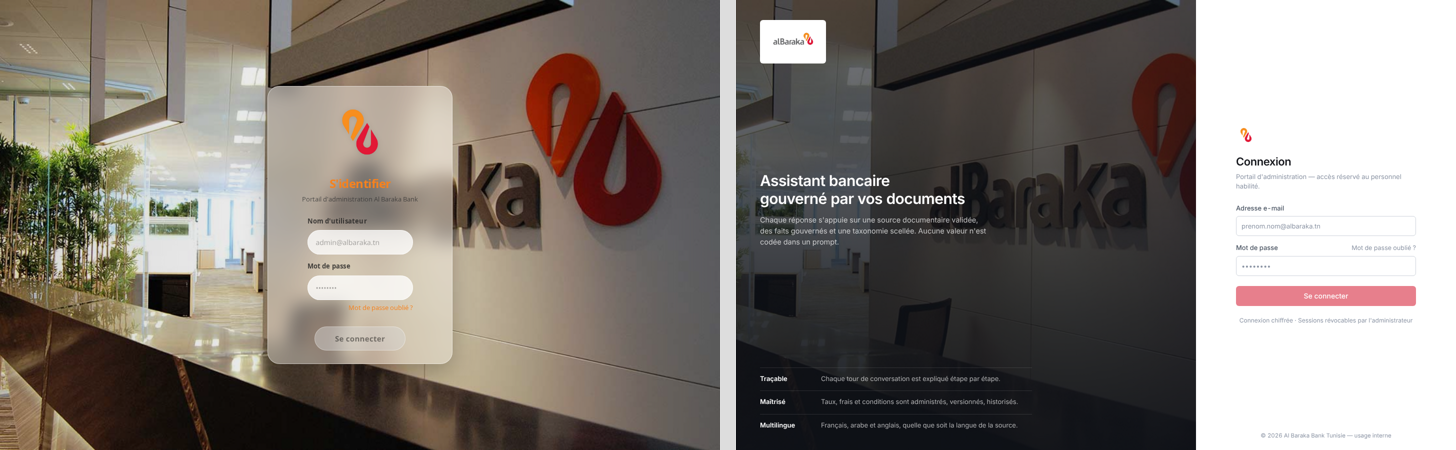
\includegraphics[width=0.96\textwidth]{assets/before-after-01-login.png}
  \caption{Portal identity: dedicated Client vs Staff login with role-based redirect.}
  \label{fig:ui}
}{
  \fbox{\parbox{0.9\textwidth}{\centering UI screenshots (assets/before-after-*.png)}}
}
\end{figure}
\begin{figure}[H]
\centering
\IfFileExists{assets/before-after-14-chat-answers.png}{
  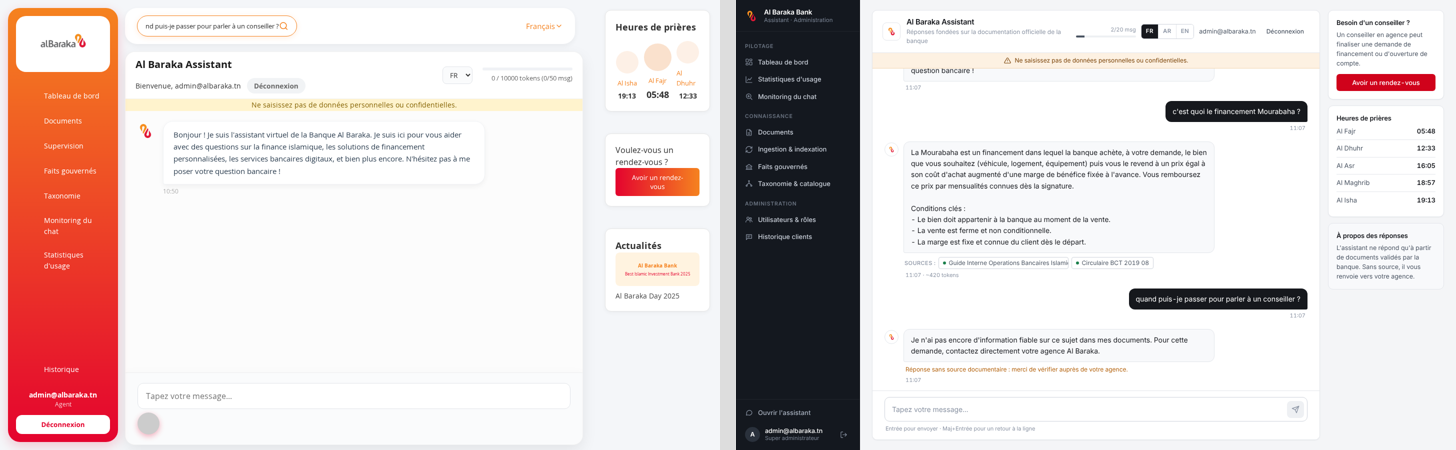
\includegraphics[width=0.96\textwidth]{assets/before-after-14-chat-answers.png}
  \caption{Chat answers: grounded responses with structured citations vs honest refusals.}
}{
  \fbox{\parbox{0.9\textwidth}{\centering Chat answer screenshots}}
}
\end{figure}

\subsection{Core Banking Data Model (V15)}

\begin{table}[H]
\centering\footnotesize
\begin{tabular}{p{3.2cm}p{11.0cm}}
\toprule
\textbf{Domain} & \textbf{Tables \& Key Fields} \\
\midrule
Identity \& Risk & \texttt{clients} (CIN, \texttt{ABK\#\#\#\#\#\#}, segment, \texttt{langue\_preferee}, KYC, risk, branch \texttt{agence\_id}) \\
Money & \texttt{comptes} (IBAN, RIB, \texttt{solde}, \texttt{decouvert\_autorise}), \texttt{cartes} (masked \texttt{porteur} e.g.\ \texttt{4571 **** **** 6842}, no PAN/CVV), \texttt{transactions} (counterparty, channel, amount) \\
Products & \texttt{financements} (\textit{murabaha/ijara}, amounts, margin, installments), \texttt{beneficiaires} (RIB, bank, country) \\
Service & \texttt{advisor\_requests} (motive, branch, date/time, free-text message) \\
Conversation & \texttt{conversations}, \texttt{public\_chat\_session}, \texttt{messages} (scrubbed Q/A, \texttt{sources\_utilisees}, \texttt{trace\_json}) \\
\bottomrule
\end{tabular}
\caption{Customer domain: realistic core-banking shape, not a toy. No full card numbers stored.}
\end{table}

\noindent Two design facts that matter: transactions may contain third-party personal data (store names), and the assistant never sees raw balances --- for a signed-in customer, a \textbf{masked context} (\texttt{CustomerContextService}) is derived at call time: slices and categories only, no direct identifiers leave the bank.

\section{Authentication, Roles and Quotas}

\begin{itemize}[leftmargin=1.2cm, itemsep=2pt]
\item \textbf{JWT with server-side rotation:} access $\leq$1h; refresh tokens carry \texttt{jti} in a \texttt{family}, single-use (\texttt{rotated}) with \textbf{reuse detection} (consumed \texttt{jti} burns the family $\rightarrow$ 401). Revocation on logout and on any admin role change / deactivation / delete.
\item \textbf{Dynamic staff roles:} \texttt{admin\_roles} + \texttt{admin\_permissions} + \texttt{role\_permission} + \texttt{admin\_access\_audit} (Flyway V14). Twelve fixed permissions; \texttt{SUPER\_ADMIN} reserved; unknown role $\rightarrow$ fail-closed 403; every change audited with mandatory reason.
\item \textbf{Two-phase metering:} \texttt{gate()} before the engine, \texttt{settle()} after. Anonymous: 3 000 tokens / 20 messages; authenticated: 10 000 / 50; max 5 new sessions/hour. Per-session \textbf{striped ReentrantLocks} (64 stripes, not \texttt{synchronized}) so a slow engine cannot be gamed --- and because the backend runs on JDK 21 virtual threads, this avoids carrier pinning.
\end{itemize}

\section{Streaming and Persistence}

\textbf{End-to-end streaming:} Python \texttt{GroqCompletion.stream} $\rightarrow$ Java \texttt{AgentClient.invokeStream} (pinned to HTTP/1.1) $\rightarrow$ Java SSE relay \texttt{POST /api/chat/message/stream} $\rightarrow$ browser \texttt{fetch + ReadableStream} parser. Fallback to classic \texttt{POST /message}; abort cleanly cancels.

\textbf{Persistence:} Java is the single writer. It opens the exchange row \textbf{before} calling RAGLab, persists after streaming, writes attribution (\texttt{engine = RAGLab}) and provenance, and sends the last \textbf{10 turns} as context to the stateless engine (\texttt{turn\_id} + \texttt{X-Turn-Id} for idempotency).

\section{Admin Console: The Control Room}

\begin{table}[H]
\centering\footnotesize
\begin{tabular}{p{4.0cm}p{10.5cm}}
\toprule
\textbf{Screen} & \textbf{Function} \\
\midrule
\texttt{/admin/facts} & Governed facts CRUD --- rates/fees/eligibility outrank any document; audit append-only \\
\texttt{/admin/taxonomy} & Exemplar \& release management; \texttt{seal()} freezes numbered release; \texttt{publish} rollback \\
\texttt{/admin/agent/health} & Effective \texttt{RAGLAB\_URL} (overridable by SUPER\_ADMIN, audited), live probe \\
\texttt{/admin/agent/quality} & Quality workbench: answer $\rightarrow$ retrieval $\rightarrow$ quote-existence, all verbatim \\
\texttt{/admin/agent/documents} & One drop zone, two chunk worlds (honest \texttt{pending/indexed/stale}) \\
\texttt{/admin/agent/config} & Models \& keys (write-only, \texttt{CONFIG\_SET} audited) --- RAGLab settings read-only \\
\texttt{/admin/agent/journal} & Every admin action, filterable by action, searchable, with motive column \\
\texttt{/admin/agent/monitor} & Live feed + KPI strip (grounded rate, refusal reasons) over last 200 exchanges \\
\bottomrule
\end{tabular}
\caption{Admin control room: every write is audited, every read is role-gated.}
\end{table}

% ══════════════════════════ CHAPTER 6 ══════════════════════════════════
\chapter{Problems Solved}\label{sec:problems}

This chapter is the heart of the internship: not what was planned, but what broke --- and what architecture prevents it from breaking again.

\begin{problembox}{Arabic PDFs Are Not Text}
\textbf{Problem:} Extracted Arabic from banking law PDFs comes out in \textbf{visual order} (right-to-left lines as rendered, not logical order), with split words, repeated gazette headers/footers, and corrupted digits. Indexed directly, the corpus is nonsense.

\textbf{Solution:} A dedicated \texttt{restructure.py} pipeline: NFKC + Arabic presentation-form repair, alef/yah unification, tatweel/diacritics stripping, page-header cleanup and repeated-header dropping ($\geq$3 occurrences), section-marker extraction (\textit{al-fasl / al-bab}), and \textbf{visual-order reconstruction by zone} into logical reading order before chunking. Linguistic repair was performed \textbf{batch by batch} (29 batches for the law: 215 corrections; then 35, 23, 21 for the other documents), each checked by \texttt{llm\_repair\_check.py} and adopted after supervisor sign-off. Raw \texttt{docs/} files are \textbf{never modified}; corrected codices are applied inside the pipeline and versioned in \texttt{raglab/audits/}.
\end{problembox}

\begin{problembox}{A 220-Token Window Destroys Meaning}
\textbf{Problem:} Fixed-window chunking (220 tokens + 40 overlap) cuts a legal article mid-definition, making the passage unverifiable.

\textbf{Solution:} Structure-aware chunking (\S4.2). Measured gain: \textbf{+20 points hit@1} (51 $\rightarrow$ 71 live; 42 $\rightarrow$ 62 offline) --- the single largest architectural win, outranking every retrieval-mode experiment.
\end{problembox}

\begin{problembox}{Searching in Arabic With French/English Questions}
\textbf{Problem:} Users write technical terms in Latin script (\textit{murabaha, sukuk}) while documents use Arabic script (\textit{مرابحة, صكوك}). Lexical search has zero overlap.

\textbf{Solution (layered):} Native multilingual embeddings (NVIDIA 2048-d) handle most cross-script cases; \textbf{declared cross-script bridges} (curated Latin$\rightarrow$Arabic equivalences, df-checked so a bridge onto boilerplate can never anchor evidence); \textbf{colloquial concept vocabulary} (e.g.\ \textit{hana/khamara/bar} $\rightarrow$ \textit{khamr}, \textit{qimar/casino} $\rightarrow$ \textit{maysir}) with scope disclosure; and one bounded \textbf{interrogation call} that rewrites a practical question into the nearest technical question.
\end{problembox}

\begin{problembox}{The Guided Retrieval Round Was Dead in Production}
\textbf{Problem:} A deployed-service bug: the sufficiency controller was called \textbf{without a search function}, so the guided rescue round never executed in production --- only in offline tests.

\textbf{Fix:} The live service now passes the search callable. This established the rule: \textit{any claim about the deployed service must be verified on the deployed service.}
\end{problembox}

\begin{problembox}{The Index Was Silently Duplicating}
\textbf{Problem:} Re-pushing an identical document created duplicates (859 of 1 713 observed), inflating term frequencies and corrupting retrieval. The legacy append-only path had no guard.

\textbf{Solutions:} RAGLab \texttt{409} content-hash guard (\texttt{document\_already\_in\_corpus}, SHA-256, not filename); batch \texttt{POST /ingest} as one-job-at-a-time (concurrent $\rightarrow$ \texttt{409} state); \texttt{POST /documents} content-hash versioning (identical bytes = no-op; different = version bump).
\end{problembox}

\begin{problembox}{French Intent Misclassified by a Substring}
\textbf{Problem:} Regex \texttt{Quelle} matched \textbf{inside} \texttt{Quelles}, misclassifying a procedural question as definitional.

\textbf{Fix:} Anchored markers + dedicated French procedural patterns, covered by live-set regression tests.
\end{problembox}

\begin{problembox}{Streaming Broke on HTTP/2 Upgrade}
\textbf{Problem:} \texttt{java.net.http.HttpClient} defaults to HTTP/2 and sends \texttt{Upgrade: h2c}; uvicorn rejected it with \texttt{422}. The browser saw a broken stream.

\textbf{Fix:} Pin \texttt{AgentClient.invokeStream} to \textbf{HTTP/1.1} explicitly. One-line cause, days of debugging.
\end{problembox}

\begin{problembox}{Two Sensitive Configuration Errors}
\textbf{Hardcoded token in Compose} overriding env + \textbf{network errors leaking as 500} (now \texttt{502} with scrubbed detail) + \textbf{nginx caching wrong \texttt{index.html}} (now no-cache + critical-CSS disabled). All three are regression-tested; the token incident was a real platform-team occurrence.
\end{problembox}

% ══════════════════════════ CHAPTER 7 ══════════════════════════════════
\chapter{Security, Privacy \& Data Governance}

\section{Defense in Depth}

\begin{table}[H]
\centering\small
\begin{tabular}{p{3.4cm}p{11.2cm}}
\toprule
\textbf{Layer} & \textbf{Mechanism} \\
\midrule
Network & Only nginx is public; backend + Postgres + RAGLab on private network; edge TLS + HSTS \\
Authentication & JWT ($\geq$256-bit, never in repo); \texttt{X-Service-Token} constant-time \texttt{hmac.compare\_digest} \\
Authorization & All admin \texttt{@PreAuthorize}; DB-backed staff permissions; client \texttt{UTILISATEUR} isolated; unknown $\rightarrow$ 403 \\
Input & Filename validation; 20\,MiB cap $\rightarrow$ 413; enum validation $\rightarrow$ 400 \\
Prompt Injection & System prompt declares Q+A as untrusted data; capability guard refuses live-data requests locally \\
Output & PII scrub \textit{after} gate: EMAIL/PHONE/RIB-IBAN/CIN $\rightarrow$ \texttt{[LABEL]} \\
Secrets & Env / platform secrets only; \texttt{GET /keys} presence + fingerprint; \texttt{POST /keys} rejects placeholders \\
\bottomrule
\end{tabular}
\caption{Security layers: each one is small; together they are complete.}
\end{table}

\section{Personal Data: What We Hold, What We Do Not}

The platform holds nine families of customer personal data across \texttt{clients}, \texttt{comptes}, \texttt{cartes}, \texttt{transactions}, \texttt{beneficiaires}, \texttt{financements}, \texttt{advisor\_requests}, \texttt{conversations}, \texttt{refresh\_tokens} --- from direct identifiers (email, CIN) to financial (IBAN/RIB) to free-text (chat, appointment messages).

\noindent\textbf{Two truths:} (1) \textit{Nothing identifiable leaves the bank} beyond a masked slice/category context built at call time for an authenticated customer; (2) \textit{The highest real risk is free text} --- a question may contain an account number; it is stored verbatim and shown to staff. The output scrub + audit mitigate; a retention/deletion lifecycle remains a documented pre-production gap with the legal team.

\noindent No full card PAN or CVV is ever stored. Transactions may contain third-party personal data (store names) --- a DPIA-relevant nuance.

\section{Audit and Traceability}

Every answer carries \texttt{citations} and engine attribution (\texttt{RAGLAB\_*}); every admin action is written to \texttt{agent\_admin\_audit} with \textbf{mandatory reason}; every ingestion writes \texttt{JournalIngestion}; every conversation is visible from its first message; monitoring KPIs (grounded rate, refusal reasons) over the last 200 exchanges attribute by engine even for historical turns.

\section{Threat Pass}

A 20-point checklist (\texttt{THREAT\_PASS\_6.2.md}) drove concrete fixes: second unauthenticated chat door removed, string compares hardened to constant-time, hardening headers at nginx + Spring, Swagger off in \texttt{prod}, host ports bound to \texttt{127.0.0.1}. Remaining documented gaps: magic-byte sniffing, per-request DB auth vs hourly rotation, Redis auth, nightly purge of expired refresh tokens.

% ══════════════════════════ CHAPTER 8 ══════════════════════════════════
\chapter{Deployment \& Operations}

\section{One Image Set, Three Environments}

\begin{table}[H]
\centering\small
\begin{tabular}{lccc}
\toprule
 & \textbf{dev} & \textbf{staging} & \textbf{prod} \\
\midrule
How & \texttt{docker compose up} & same images, real TLS & same images, HA stores \\
Profile & (default) & \texttt{prod} & \texttt{prod} \\
Swagger & on & off & off \\
Logs & plain / json & ecs & ecs \\
Secrets & \texttt{.env} (local) & platform secrets & platform secrets \\
Data & throwaway & anonymized monthly & live \\
\bottomrule
\end{tabular}
\caption{Promotion moves image digests dev $\rightarrow$ staging $\rightarrow$ prod; never rebuild for prod.}
\end{table}

\noindent \texttt{deploy/promote.sh} enforces it: refuses a dirty tree, tags with commit SHA (never \texttt{latest}), and \texttt{verify} compares \texttt{GET /actuator/info} + \texttt{GET /version.json} against \texttt{HEAD}.

\section{Topology}

\begin{center}
\small\texttt{Internet --443(TLS,HSTS)--> Edge Proxy --80(private)--> nginx SPA --/api--> Spring Boot --> RAGLab (private)}\\
\small\texttt{|--> Postgres (PITR: daily full + WAL, 30-day retention, quarterly drill)}
\end{center}

\noindent Postgres is managed-service where available; Flyway runs at backend boot. \texttt{docker-compose.prod.yml} (per host) sets \texttt{prod} profile, removes host port mappings, and points at secret files. Kubernetes translation is one-to-one.

\section{Deploy Procedure}

\begin{verbatim}
TAG=v1.0.0 docker compose -f docker-compose.yml \
                         -f docker-compose.prod.yml pull
docker compose -f docker-compose.yml \
               -f docker-compose.prod.yml up -d backend
docker compose logs backend | grep -E "Flyway|Migrating|Successfully"
docker compose -f docker-compose.yml \
               -f docker-compose.prod.yml up -d frontend
E2E_BASE_URL=https://assistant.example.tn ./e2e/run.sh
\end{verbatim}

\section{Observability}

\textbf{Correlation:} \texttt{turnId} minted once in Java, sent as body + \texttt{X-Turn-Id}, bound to MDC and Python \texttt{contextvar} --- one grep spans both services; \texttt{X-Request-Id} echoed.

\textbf{Metrics:} backend \texttt{GET /actuator/prometheus} $\rightarrow$ \texttt{chat\_turns\_total / chat\_turn\_duration}; Python \texttt{GET /metrics} $\rightarrow$ \texttt{agent\_turns\_total / agent\_answer\_chars\_total}. OpenTelemetry tracing is the documented next step.

\noindent\textit{Runbooks:} \texttt{RUNBOOK.md} covers incidents, ingestion, rotation, regulatory audit queries. \texttt{HOST\_TESTING.md} + \texttt{docker-compose.test.yml} give a one-command full-stack test on a workstation.

% ══════════════════════════ CHAPTER 9 ══════════════════════════════════
\chapter{Results, Evaluation \& Limitations}

\section{How Quality Is Measured}

Two frozen question sets anchor every claim:

\begin{itemize}[leftmargin=1.2cm, itemsep=2pt]
\item \textbf{\texttt{questions\_50.json}} --- 50 cases: 10 verbatim, 20 paraphrases, 15 cross-lingual (6 FR + 9 EN), 5 out-of-scope. 32 AR / 8 FR / 10 EN. Expected document + substring verified as distinctive.
\item \textbf{\texttt{questions\_targets.json}} --- 10 Arabic cases: 2 per category (colloquial, synonyms, implicit, compound, ambiguity).
\end{itemize}

\noindent\textbf{Rules:} paired comparison in same run; $\pm$2\,pp tolerance across runs; a frozen set is never edited to improve a result; offline BM25 filters cheaply, live runs decide.

\section{Headline Results}

\begin{table}[H]
\centering\footnotesize
\begin{tabular}{p{5.6cm}p{8.6cm}}
\toprule
\textbf{What} & \textbf{Result} \\
\midrule
Chunking (live vector, 50 cases) & \texttt{size} 51/64/71 $\rightarrow$ \textbf{restructure 71/80/87} (hit@1/3/5) --- +20\,pp \\
Retrieval modes (restructure) & dense \textbf{71/80/87} $>$ RRF 71/80/82 $>$ blend 62/80/84 --- dense default \\
Reranker (offline) & 62/82/87 $\rightarrow$ \textbf{62/89/89} --- activated \\
Knowledge unit index (law) & 67/92/92 $\rightarrow$ \textbf{100/100/100} --- every article at rank 1 \\
Target categories (10, dense) & compound 100/100/100 $\cdot$ implicit+ambiguous 50/100/100 $\cdot$ synonyms 50 $\cdot$ colloquial 0 (addressed via vocabulary) \\
Model independence (2 LLMs, same retrieval) & agreement \textbf{0.720}; Jaccard of sources \textbf{1.000} --- divergence is accept/refuse, not which source \\
Final campaign (7+12+6 live) & retrieval 5/7 $\cdot$ topic map 5/5 $\cdot$ end-to-end 3 answered / 3 refused, zero errors, k=5/12/20 no change \\
Robustness (6 adversarial) & Fabricated/borrowed/computed/unknown-marker/injection --- all rejected deterministically \\
Tests & 472 unit + 133 offline checks $\cdot$ 8 CI workflows $\cdot$ 469 hard-harness families \\
\bottomrule
\end{tabular}
\caption{Results that are measured, not claimed. All numbers from frozen artifacts.}
\end{table}

\section{What the System Does Not Do (Yet)}

\begin{table}[H]
\centering\footnotesize
\begin{tabular}{p{4.8cm}p{9.6cm}}
\toprule
\textbf{Limitation} & \textbf{Scope} \\
\midrule
Citation existence $\neq$ entailment & Gate proves words/numbers come from source, not that claim follows logically \\
No similarity threshold & Top-5 transmitted even if off-topic; safety rests on sufficiency + refusal \\
Single worker & One profile/index/ingest at a time; horizontal scale is designed, not deployed \\
Updates by re-ingestion & Old fragments serve until next ingest (now surfaced as \texttt{stale}) \\
Tokenizer variance & Without \texttt{cl100k} vocab, boundaries differ --- only CI is authoritative \\
Evaluation scale & 50 + 10 cases small \& correlated --- not a security/legal guarantee \\
\bottomrule
\end{tabular}
\end{table}

\begin{center}
\small\color{abarakaRed}\textbf{Suitable for a supervised pilot on approved non-confidential documents; not ready for unsupervised customer-facing banking advice.} --- as stated in the repository itself.
\end{center}

% ══════════════════════════ CHAPTER 10 ══════════════════════════════════
\chapter{Conclusion \& Perspectives}

\section{What Was Built}

A working, documented and measurable platform: a complete language pipeline (reading and repair, structure-aware chunking, vector + lexical indexing, dense retrieval, intent and sufficiency reasoning, citation-gated generation, output scrubbing, audit) wrapped in a bank-operated web app that owns identity, quotas and persistence --- all measured, versioned and traceable.

\section{Lessons That Outlive the Code}

\begin{enumerate}[leftmargin=1.2cm, itemsep=4pt]
\item \textbf{Measurement replaces opinion.} Every structural choice --- restructure over window, dense over fusion, lexicon off, relational expansion abandoned --- was settled by paired numbers, and several reasonable intuitions were rejected by data.
\item \textbf{Governance of decisions is architecture.} The step-and-plan protocol, activation gates and frozen question sets allowed the project to survive interruptions without silent regression and to distinguish progress from displacement.
\item \textbf{Reality is the only judge.} The most expensive defects --- the inert guided round, the French intent misclassification, index duplication --- were invisible in tests and obvious in operation. Any claim about the deployed service must be checked on the deployed service.
\end{enumerate}

\section{Next Steps}

\begin{enumerate}[leftmargin=1.2cm, itemsep=2pt]
\item \textbf{Per-document authorization} and chunk-level topical metadata (\texttt{path / level / parent\_id}) before any production re-index.
\item \textbf{Topical \& faceted retrieval arms} measured on frozen sets, fused with dense --- without reintroducing known regressions.
\item \textbf{Closing measurement campaign} --- re-measure every arm, document limits, then decide defaults.
\item \textbf{Industrialization:} multi-user semantics, incremental updates, observability (metrics + tracing), adversarial evaluation, upload magic-byte validation, OpenTelemetry, and a legal-team-reviewed retention/deletion lifecycle.
\item \textbf{Product:} safely editable answer templates and conversation quality flags in the control room.
\end{enumerate}

\vspace{0.6cm}
\begin{center}
\begin{tcolorbox}[colback=softGray, colframe=chapterBlue!20, boxrule=0.5pt, arc=4pt, width=13cm]
\centering\small
\color{textDark!85}\textit{``The best system we built is not the one that answers the most questions,\\ but the one that knows when not to answer --- and can prove why.''}\\[3pt]
\footnotesize\color{espritNavy!70} --- Farah AYARI, ESPRIT $\cdot$ \CompanyName\ --- \CompanySite\ --- supervised by \SupervisorName
\end{tcolorbox}
\end{center}

% ── References ─────────────────────────────────────────────────────────
\chapter*{References}
\addcontentsline{toc}{chapter}{References}
\small

All references are repository-internal (no external browsing needed to verify numbers):

\begin{table}[H]
\centering\footnotesize
\begin{tabular}{p{6.0cm}p{8.4cm}}
\toprule
\textbf{Document} & \textbf{Content} \\
\midrule
\texttt{RAGLab/README.md} & Supported pipeline, measured A/B tables \\
\texttt{RAGLab/RAGLAB\_SPEC.md} & Reverse-engineered specification \\
\texttt{RAGLab/RAGLAB\_GAP\_ANALYSIS.md} & Target-state gap analysis \\
\texttt{RAGLab/RAGLAB\_ROADMAP.md} & Binding execution plan \\
\texttt{RAGLab/raglab/CONTRACT.md} & Frozen HTTP contract \\
\texttt{RAGLab/raglab/SERVICE.md} & Service operation guide \\
\texttt{bank-assistant/README.md} & Web-app overview \& governance model \\
\texttt{bank-assistant/PLAN\_TO\_PROD.md} & Phased plan (phases 0 $\rightarrow$ 10) \\
\texttt{bank-assistant/docs/DEPLOYMENT.md} & Deployment topology \\
\texttt{bank-assistant/docs/CUSTOMER\_PII\_REPORT.md} & Customer PII inventory \\
\texttt{bank-assistant/docs/THREAT\_PASS\_6.2.md} & 20-point security checklist \\
\texttt{RAGLab/docs/} (4 real docs) & Law 2016-48, BCT Circular, Guide, \textit{Madkhal} \\
\bottomrule
\end{tabular}
\end{table}

\noindent\textit{Institutional context consulted:} Al Baraka Bank Tunisia official site (history, 44 branches, IFN Awards); Law 2016-48, Official Journal No.\ 58 of 15 July 2016; ESPRIT (Ariana, 2003, CTI EUR-ACE 2023).

% ── Appendices ─────────────────────────────────────────────────────────
\appendix
\chapter{Glossary}

\begin{table}[H]
\centering\small
\begin{tabular}{p{4.2cm}p{3.4cm}p{6.6cm}}
\toprule
\textbf{Term} & \textbf{Transliteration} & \textbf{Meaning} \\
\midrule
المرابحة & \textit{al-murabaha} & Cost-plus sale with disclosed capital and margin \\
الإجارة & \textit{al-ijara} & Lease with acquisition option \\
الصيغة & \textit{al-sigha} & Contractual form (offer \& acceptance) \\
الفصل & \textit{al-fasl} & Article (law) / chapter (circular) \\
نافذ & \textit{nafidh} & In force \\
كافٍ & \textit{kafin} & Sufficient (evidence) \\
غير كافٍ & \textit{ghayr kafin} & Insufficient \\
متعارض & \textit{muta`arid} & Contradictory \\
RAG & --- & Retrieval-Augmented Generation \\
hit@k & --- & Expected document/fragment in top-k \\
RRF & --- & Reciprocal Rank Fusion \\
BM25 & --- & Lexical ranking function \\
Citation gate & --- & Quote membership + numeric gate \\
Sufficiency & --- & Whether evidence satisfies the proof plan \\
Gate / Porte & --- & Feature flag with byte-identical rollback \\
\bottomrule
\end{tabular}
\end{table}

\emph{Note: Arabic terms are transliterated here so the file compiles with pdflatex without Arabic fonts; the Markdown version and the PDF's narrative preserve the original script where the font allows it.}

\chapter{Key Figures}

\begin{table}[H]
\centering\small
\begin{tabular}{p{5.4cm}p{8.8cm}}
\toprule
\textbf{Fact} & \textbf{Source} \\
\midrule
RAGLab: 376 commits $\cdot$ 249 files $\cdot$ 86 Python modules & Git history \& \texttt{RAGLAB\_FULL\_REPORT.md} \\
Corpus: 4 docs $\rightarrow$ 339 fragments (233/54/39/13) & \texttt{raglab/audits/MASTER\_INDEX.md} \\
Tests: 472 unit + 133 offline $\cdot$ 8 workflows & CI at merge (\texttt{service v1.5.0}) \\
Web app: 255 commits $\cdot$ 428 files $\cdot$ 15 migrations & \texttt{bank-assistant/docs/PROJECT\_REPORT.md} \\
Stack: NVIDIA 2048-d + xKiro Qwen (pinned, no fallback) & \texttt{raglab/pipeline\_policy.py} \\
\bottomrule
\end{tabular}
\end{table}

\chapter{Reproduction}

\begin{verbatim}
# RAGLab
cd RAGLab/raglab
python3 -m venv .venv && source .venv/bin/activate
pip install -r requirements.txt
./run_tests.sh --offline
python main.py ingest --reset --data-dir ../docs
python main.py answer "..." --query-lang ar

# Web app (Docker)
cp bank-assistant/.env.docker.example .env
# set RAGLAB_URL, RAGLAB_TOKEN, JWT_SECRET
docker compose up --build   # http://localhost:8080

# Verify
curl http://localhost:8000/health
curl http://localhost:8080/api/agent/health \
     -H "Authorization: Bearer <token>"
\end{verbatim}

\vspace{1cm}
\begin{center}
\small\emph{Report prepared by \StudentName{} --- ESPRIT, internship at \CompanyName{} --- \CompanySite, supervised by \SupervisorName.}\\[3pt]
\footnotesize\color{textDark!65} This document contains no account identifiers, repository URLs or credentials. All figures are traceable to the two repositories and their frozen benchmark artifacts.
\end{center}

\end{document}
